\documentclass[aspectratio=169]{beamer}
\usetheme{Boadilla}
%\usetheme{Warsaw}
%\setbeamercovered{transparent}
\beamertemplatetransparentcoveredhigh
\usepackage[portuges]{babel}
\usepackage[utf8]{inputenc}
\usepackage{lmodern}
\usepackage[T1]{fontenc}
\usepackage[portuguese, linesnumbered, vlined, titlenumbered, ruled]{algorithm2e}
\SetKwRepeat{Registro}{registro \{}{\}}%
\usepackage{hyperref} 

% Macro que faz com que a numeracao de diferentes algoritmos continue de onde parou
\newcommand{\rememberlines}{\xdef\rememberedlines{\number\value{AlgoLine}}}
\newcommand{\resumenumbering}{\setcounter{AlgoLine}{\rememberedlines}}


\title[Aula Prática - Árvores B]{Algoritmos e Estrutura de Dados}
\subtitle{Árvores B}
\author[Frederico Santos de Oliveira]{prof. Frederico Santos de Oliveira}
\institute[UFMT]{Universidade Federal de Mato Grosso\\ Faculdade de Engenharia}
\date{}

\begin{document}

\begin{frame}
\titlepage % Print the title page as the first slide

\begin{figure}[!h]
  \centering
   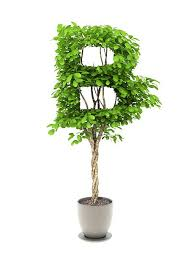
\includegraphics[width=80pt]{imagens/introducao.jpg}
  \label{fig_introducao}
\end{figure}
\end{frame}

%\section*{Roteiro}

\begin{frame}
  \frametitle{Agenda}
  \tableofcontents
\end{frame}

%%%%%%%%%%%%%%%%%%%%%%%%%%%%%%%%%%%%%%%%%%%%%%%%%%%%%%%%%%%%%%%%%%%%%%%%%%%%%%%%%%%%%%%%%%%%%%%%%%%
\section{Introdução}
%%%%%%%%%%%%%%%%%%%%%%%%%%%%%%%%%%%%%%%%%%%%%%%%%%%%%%%%%%%%%%%%%%%%%%%%%%%%%%%%%%%%%%%%%%%%%%%%%%%


%%%%%%%%%%%%%%%%%%%%%%%%%%%%%%%%%%%%%%%%%%%%%%%%%%%%%%%%%%%%%%%%%%%%%%%%%%%%%%%%%%%%%%%%%%%%%%%%%%%
\subsection{Estrutura Nodo}
%%%%%%%%%%%%%%%%%%%%%%%%%%%%%%%%%%%%%%%%%%%%%%%%%%%%%%%%%%%%%%%%%%%%%%%%%%%%%%%%%%%%%%%%%%%%%%%%%%%

\begin{frame}[fragile]{Árvore B}{Estrutura Nodo}
\begin{algorithm}[H]
\caption{Nodo} 
\label{Nodo}
\Inicio{
 \Registro{Nodo}{
    Vetor Inteiro: key[1..2t-1]; \CommentSty{// Vetor de chaves.}\\
    Vetor Ponteiro Nodo: c[1..2t]; \CommentSty{// Vetor de ponteiros.} \\
    Inteiro: n; \CommentSty{// Quantidade de chaves armazenadas.} \\
    Booleano: folha; \CommentSty{// Indica se o nodo é folha.}
  }
}
\end{algorithm} 
\end{frame}

%%%%%%%%%%%%%%%%%%%%%%%%%%%%%%%%%%%%%%%%%%%%%%%%%%%%%%%%%%%%%%%%%%%%%%%%%%%%%%%%%%%%%%%%%%%%%%%%%%%
\section{Operações Básicas}
%%%%%%%%%%%%%%%%%%%%%%%%%%%%%%%%%%%%%%%%%%%%%%%%%%%%%%%%%%%%%%%%%%%%%%%%%%%%%%%%%%%%%%%%%%%%%%%%%%%

\begin{frame}{Operações Básicas}
A seguir, as operações básicas a serem realizadas sobre Árvores B:
 \begin{itemize}
 \item ArvoreB-Criar
 \item ArvoreB-Busca
 \item ArvoreB-Inserir
 \item ArvoreB-Remover
\end{itemize}
\end{frame}

%%%%%%%%%%%%%%%%%%%%%%%%%%%%%%%%%%%%%%%%%%%%%%%%%%%%%%%%%%%%%%%%%%%%%%%%%%%%%%%%%%%%%%%%%%%%%%%%%%%
\subsection{Criar}
%%%%%%%%%%%%%%%%%%%%%%%%%%%%%%%%%%%%%%%%%%%%%%%%%%%%%%%%%%%%%%%%%%%%%%%%%%%%%%%%%%%%%%%%%%%%%%%%%%%

\begin{frame}{CriaÁrvore}{Pseudocódigo}
% \scalebox{0.8}{
\begin{algorithm}[H]
\caption{ArvoreB-Criar} 
\label{B-Tree-Create}
\Entrada{Ponteiro $T$ para a árvore.}
\Inicio{
  novo $\leftarrow$ ALOCA\_NODO() \\
  novo.folha $\leftarrow$ TRUE \\
  novo.n $\leftarrow$ 0 \\
  DISK\_WRITE(novo) \\
  T.raiz $\leftarrow$ novo
}
\end{algorithm}
\tiny{Adaptado de \cite{Cormen2012}.}
% }  
\begin{itemize}
 \item ALOCA\_NODO() aloca uma página no disco de modo a ser usada como um novo nodo.
 \item Requer $O(1)$ operações no disco e tempo de processador $O(1)$.
\end{itemize}
\end{frame}

%%%%%%%%%%%%%%%%%%%%%%%%%%%%%%%%%%%%%%%%%%%%%%%%%%%%%%%%%%%%%%%%%%%%%%%%%%%%%%%%%%%%%%%%%%%%%%%%%%%
\subsection{Busca}
%%%%%%%%%%%%%%%%%%%%%%%%%%%%%%%%%%%%%%%%%%%%%%%%%%%%%%%%%%%%%%%%%%%%%%%%%%%%%%%%%%%%%%%%%%%%%%%%%%%

\begin{frame}{Busca}{Pseudocódigo}
\scalebox{0.9}{
\begin{algorithm}[H]
\caption{ArvoreB-Busca} 
\label{B-Tree-Search}
\Entrada{Ponteiro para a raiz $r$, chave $k$ a ser buscada na árvore.}
\Saida{O nodo que contém $k$ ou NULL caso não encontre.}
\Inicio{
  i$\leftarrow$ 1 \\
  \Enqto{($i \leq r.n$) e ($k > r.key[i]$)} {
    $i \leftarrow i + 1$ \\ 
  }
  \Se {($i\leq r.n$) e ($k = r.key[i]$)} {
    \Retorna (r, i)
  }
  \Se {r.folha} {
    \Retorna NULL
  }
  \Senao { 
    DISK\_READ($r.c_i$) \\
    \Retorna ArvoreB-Busca($r.c[i]$, k)
  }
}
\end{algorithm}
}  

\tiny{Adaptado de \cite{Cormen2012}}.
\end{frame}


%%%%%%%%%%%%%%%%%%%%%%%%%%%%%%%%%%%%%%%%%%%%%%%%%%%%%%%%%%%%%%%%%%%%%%%%%%%%%%%%%%%%%%%%%%%%%%%%%%%
\subsection{Inserção}
%%%%%%%%%%%%%%%%%%%%%%%%%%%%%%%%%%%%%%%%%%%%%%%%%%%%%%%%%%%%%%%%%%%%%%%%%%%%%%%%%%%%%%%%%%%%%%%%%%%

\begin{frame}{Divisão}{Pseudocódigo}
\scalebox{0.9}{
\begin{algorithm}[H]
\caption{ArvoreB-Divide-Filho} 
\label{B-Tree-Split-CHild}
\Entrada{Um nodo interno não-cheio $x$, um índice $i$, um nodo cheio $y$ filho de $x$, tal que $y=x.c_i$.}
\Inicio{  
  z $\leftarrow$ ALOCA\_NODO() \label{divide_filho_aloca_z_inicio}\\
  z.folha $\leftarrow$ y.folha \\
  z.n $\leftarrow$ t-1 \label{divide_filho_aloca_z_fim} \\
  \Para {($j\leftarrow 1$ \textrm{ até } t-1)} { \label{divide_filho_aloca_copia_inicio}
    $z.key[j] \leftarrow y.key[j+t]$ \\
  }\label{divide_filho_aloca_copia_fim}
  \Se {(NOT(y.folha))} { \label{divide_filho_aloca_copia_c_inicio}
    \Para {($j \leftarrow 1$ \textrm{ até } t)} {
      $z.c[j] \leftarrow y.c[j+t]$ \\     
    }
  } \label{divide_filho_aloca_copia_c_fim}
  y.n $\leftarrow$ t-1 \label{divide_filho_atualiza_y} \\
  \rememberlines
}
\end{algorithm}
}

\tiny{Adaptado de \cite{Cormen2012}.}  
\end{frame}

%%%%%%%%%%%%%%%%%%%%%%%%%%%%%%%%%%%%%%%%%%%%%%%%%%%%%%%%%%%%%%%%%%%%%%%%%%%%%%%%%%%%%%%%%%%%%%%%%%%\textbf{•}

\begin{frame}{Divisão}{Pseudocódigo}
\scalebox{0.9}{
\begin{algorithm}[H]
\caption{ArvoreB-Divide-Filho (continuação)} 
\label{B-Tree-Create2}
\resumenumbering
\Inicio{
  \Para {($j\leftarrow x.n+1$ \textrm{ descendo até } $i+1$)} { \label{divide_filho_move_x_inicio}
    $x.c[j+1] \leftarrow x.c[j]$ \\
  } \label{divide_filho_move_x_fim}
  $x.c[i+1] \leftarrow z$ \label{divide_filho_atualiza_filho_z} \\
  \Para {($j\leftarrow x.n$ \textrm{ descendo até } $i$)} { \label{divide_filho_move_chave_x_inicio}
    $x.key[j+1] \leftarrow x.key[j]$ \\
  } \label{divide_filho_move_chave_x_fim}
  $x.key[i] \leftarrow y.key[t]$ \label{divide_filho_adiciona_chave_x} \\ 
  $x.n \leftarrow x.n + 1$ \label{divide_filho_atualiza_x} \\
  DISK\_WRITE(y)\\
  DISK\_WRITE(z)\\
  DISK\_WRITE(x)\\
}
\end{algorithm}
}

\tiny{Adaptado de \cite{Cormen2012}.}
\end{frame}

%%%%%%%%%%%%%%%%%%%%%%%%%%%%%%%%%%%%%%%%%%%%%%%%%%%%%%%%%%%%%%%%%%%%%%%%%%%%%%%%%%%%%%%%%%%%%%%%%%%

\begin{frame}{Inserção}{Pseudocódigo}
\scalebox{0.8}{
\begin{algorithm}[H]
\caption{ArvoreB-Inserir} 
\label{B-Tree-Insert}
\Entrada{Ponteiro $T$ para a árvore, chave $k$ a ser inserida.}
\Inicio{
  r $\leftarrow$ T.raiz \\ 
  \Se {($r.n = 2t-1$)} {
    s $\leftarrow$ ALOCA\_NODO() \\
    T.raiz $\leftarrow$ s\\
    s.folha $\leftarrow$ FALSE \\
    s.n $\leftarrow$ 0\\
    $s.c[i] \leftarrow$ r \\
    ArvoreB-Divide-Filho(s,1,r) \\
    ArvoreB-Inserir-NaoCheio(s,k) \\
  }
  \Senao {
    ArvoreB-Inserir-NaoCheio(r,k) \\
  }
}
\end{algorithm}
}

\tiny{Adaptado de \cite{Cormen2012}.}
\end{frame}

%%%%%%%%%%%%%%%%%%%%%%%%%%%%%%%%%%%%%%%%%%%%%%%%%%%%%%%%%%%%%%%%%%%%%%%%%%%%%%%%%%%%%%%%%%%%%%%%%%%

\begin{frame}{Inserção}{Pseudocódigo}
\scalebox{0.55}{
\begin{algorithm}[H]
\caption{ArvoreB-Inserir-NaoCheio} 
\label{B-Tree-Insert-Non-Ful}
\Entrada{Nodo raiz $x$, chave $k$ a ser inserida.}
\Inicio{
  i $\leftarrow$ x.n \\ 
  \Se {($x.folha$)} {
    \Enqto{($i \geq 1$) e ($k < x.key[i]$)} { \label{insere_naocheio_desloca_chaves_x_inicio}
      $x.key[i+1] \leftarrow x.key[i]$ \\
      i $\leftarrow$ i - 1 \\      
    }
    $x.key[i+1] \leftarrow k$ \\
    x.n $\leftarrow$ x.n + 1 \\
    DISK\_WRITE(x)\label{insere_naocheio_desloca_chaves_x_fim}\\
  }
  \Senao { \label{insere_naocheio_nao_folha_inicio}
    \Enqto{($i \geq 1$) e ($k < x.key[i]$)} {
      i $\leftarrow$ i - 1 \\    
     }
     i $\leftarrow$ i + 1 \label{insere_naocheio_nao_folha_fim}\\
     DISK\_READ($x.c[i]$) \\
     \Se {($x.c[i].n = 2t - 1$)} { \label{insere_naocheio_filho_cheio}
	B-Tree-Split-Child(x,i,$x.c[i]$)\label{insere_naocheio_divide_filho}\\
	\Se {($k > x.key[i]$)} { \label{insere_naocheio_determina_posicao_inicio}
	  i $\leftarrow$ i + 1 \label{insere_naocheio_determina_posicao_fim} \\
	}
     }
     ArvoreB-Inserir-NaoCheio($x.c[i]$, k)\\
  }
}
\end{algorithm}
}

\tiny{Adaptado de \cite{Cormen2012}.}
\end{frame}

%%%%%%%%%%%%%%%%%%%%%%%%%%%%%%%%%%%%%%%%%%%%%%%%%%%%%%%%%%%%%%%%%%%%%%%%%%%%%%%%%%%%%%%%%%%%%%%%%%%
\subsection{Remoção}
%%%%%%%%%%%%%%%%%%%%%%%%%%%%%%%%%%%%%%%%%%%%%%%%%%%%%%%%%%%%%%%%%%%%%%%%%%%%%%%%%%%%%%%%%%%%%%%%%%%

\begin{frame}{Remoção}
Considere $k$ a chave a ser removida e $x$ o nodo que contém $k$. Existem três casos:
 \begin{enumerate}[(1)]
  \item Se a chave $k$ está em $x$, um nodo folha, e $x$ contém pelo menos $t$ chaves. 
  \begin{itemize}
  \item A remoção é trivial.
  \end{itemize}
  \item Se a chave $k$ está em $x$, um nodo interno. Existem três casos a considerar:
  \begin{enumerate}[(a)]
  \item Verifique se o filho à esquerda $y$ possui pelo menos $t$ chaves. Nesse caso, a chave predecessora $k'$ de $k$ é movida para $x$, e em seguida remove-se $k$.
  \item Simetricamente, verifique se o filho à direita $z$ possui pelo menos $t$ chaves. Nesse caso, a chave sucessora $k'$ de $k$ é movida para $x$, e em seguida remove-se $k$. 
  % \item Se o filho $y$ que precede $k$ no nodo $x$ tem no mínimo $t$ chaves (mais que o mínimo), então encontre a chave predecessora $k'$ na subárvore enraizada em $y$. Recusrivamente remova $k'$ e substitua $k$ por $k'$ em $x$.
  %\item Simetricamente, se o filho $z$ que sucede $k$ no nodo $x$ tem no mínimo $t$ chaves (mais que o mínimo), então encontre a chave sucessora $k'$ na subárvore enraizada em $z$  e substitua como no anterior.
  \item Caso contrário, se ambos $y$ e $z$  tem apenas $t-1$ chaves, realize a união de $k$.
  \begin{itemize}
  \item Todos os elementos em $z$ e em $y$ passam a pertencer a um único nodo, em conjunto com a chave $k$. 
  \item Com isso, $k$ e o ponteiro para $z$ são removidos de $x$. $y$ agora contém $2t-1$ chaves, e subsequentemente $k$ é removida.
  \end{itemize} 
  \end{enumerate} 
 \end{enumerate}
\end{frame}

%%%%%%%%%%%%%%%%%%%%%%%%%%%%%%%%%%%%%%%%%%%%%%%%%%%%%%%%%%%%%%%%%%%%%%%%%%%%%%%%%%%%%%%%%%%%%%%%%%%

\begin{frame}{Remoção}
 \begin{enumerate}[(3)]
  \item Se a chave $k$ não foi encontrada no nodo $x$. 
  \begin{itemize}
    \item É necessário determinar a subárvore $x.c[i]$ apropriada que deve conter $k$.
  \end{itemize}
  \begin{enumerate}[(a)]
  \item Ao determinar o filho que contém $k$, verifica-se se este possui apenas $t-1$ chaves.
  \begin{itemize}
  \item Verifique se um dos irmãos de $x.c[i]$ possui pelo menos $t$ chaves. Se possível, movimente uma chave do irmão à esquerda ou à direita para $x$.
  \item Se  $x.c[i]$ tiver filhos, verifique também se um deles possui pelo menos $t$ chaves. Nesse caso, movimente uma chave de um filho.
  \end{itemize}
  \item Caso contrário, $x.c[i]$, todos os seus filhos e irmãos contém apenas $t-1$ chaves. Dessa forma, resta apenas fazer a intercalação de $x.c[i]$ com um de seus irmãos, o que envolve mover uma chave de $x$ para baixo.
  \end{enumerate} 
 \end{enumerate}
\end{frame}

%%%%%%%%%%%%%%%%%%%%%%%%%%%%%%%%%%%%%%%%%%%%%%%%%%%%%%%%%%%%%%%%%%%%%%%%%%%%%%%%%%%%%%%%%%%%%%%%%%%

%\begin{frame}
%\Huge{\centerline{Dúvidas?}}
%
%\begin{figure}[!h]
%  \centering
%  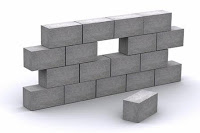
\includegraphics[width=100pt]{imagens/duvidas.jpg}
%  \label{fig_fim}
%\end{figure}
%\end{frame}

%%%%%%%%%%%%%%%%%%%%%%%%%%%%%%%%%%%%%%%%%%%%%%%%%%%%%%%%%%%%%%%%%%%%%%%%%%%%%%%%%%%%%%%%%%%%%%%%%%%
 
\section{Referências bibliográficas}
  \frame{\frametitle{Referências Bibliográficas}
    \bibliographystyle{abntex2-alf}
    \bibliography{referencias}
 }
  
%%%%%%%%%%%%%%%%%%%%%%%%%%%%%%%%%%%%%%%%%%%%%%%%%%%%%%%%%%%%%%%%%%%%%%%%%%%%%%%%%%%%%%%%%%%%%%%%%%%

\begin{frame}{Material Complementar}
Animações
\begin{itemize}
\item \href{https://www.cs.usfca.edu/~galles/visualization/BTree.html}{https://www.cs.usfca.edu/~galles/visualization/BTree.html}
\begin{itemize}
\item Obs.: Escolha "Max Degree = $4^n$ para árvore de ordem $t=2$.
\end{itemize}
\item \href{http://cs.armstrong.edu/liang/animation/web/24Tree.html}{http://cs.armstrong.edu/liang/animation/web/24Tree.html}
\begin{itemize}
\item Árvore 2-3-4
\end{itemize}
\end{itemize}
\end{frame}

%%%%%%%%%%%%%%%%%%%%%%%%%%%%%%%%%%%%%%%%%%%%%%%%%%%%%%%%%%%%%%%%%%%%%%%%%%%%%%%%%%%%%%%%%%%%%%%%%%%

\end{document}
